\documentclass{article}
\usepackage[utf8]{inputenc}
\usepackage{array}
\usepackage{amsmath,amssymb}
\usepackage{booktabs}
\usepackage{caption}
\usepackage[nodayofweek]{datetime}
\usepackage{environ}
\usepackage{float}
\usepackage{enumitem}
\usepackage{fancyhdr}
\usepackage[margin=25mm,footskip=1pt,includefoot]{geometry}
\usepackage{graphicx}
\usepackage{hyperref}
\usepackage{multicol}
\usepackage{rotating}
\usepackage{tikz}
\usepackage{threeparttable}
\usepackage{url}
\usepackage{xspace}
\usepackage{bm}
\usepackage{lipsum}


\hypersetup{
    colorlinks=true,
    urlcolor=blue}

\begin{document}
\noindent
\textbf{ES280 Problem Set 2} \\
\textbf{Nick Normandin} \\
\section*{Classmates consulted}

\section{Uniform colors}%
\label{sec:Uniform colors}

\subsection{One-sided vs. two-sided tests}%
The researchers would likely use a two-sided test in this case because they do not appear to have a prior belief about one color having a higher probability of winning than the other. They state that the problem is to determine whether "one of the colors will win a majority of the time", which indicates that they are looking for any deviation from the expected probability of $0.5$. One implication of using a two-sided test is that it will increase the p-value.
\label{sub:One-sided vs. two-sided tests}
\begin{enumerate}[label=\alph*.]
    \item The null hypothesis $H_0$ is that the probability of a competitor wearing red winning is equal to $0.5$. The alternative hypothesis $H_a$ is that the probability of the competitor wearing red winning is greater than $0.5$.
    \item $H_0: p = 0.5, \quad H_a: p > 0.5$
    \item Since the number of samples is large ($n>>40$) we will use the Z statistic. 
        $$Z = \frac{\hat{P} - p - \Delta_\mu}{\sqrt{p(1-p)/n}}=\frac{0.543 - 0.5 - 0}{\sqrt{0.5(1-0.5)/457}}=1.82$$
    \item We could use a binomial distribution (a series of coin flips) to simulate this same experiment. We could flip a fair coin ($p(heads)=0.5$) 457 times and count the number of heads (successes). We could run this simulation thousands of times, creating an empirical PMF out of the proportion of successes observed. We could then sum the portion of the PMF that is as or more extreme than a success rate (rate of seeing heads) $54.3\%$ of the time. Since the number of heads out of 457
        flips is countably finite, we could use a discrete distribution.
    \item Entering \texttt{1-normcdf(1.82)} into Matlab yields a p-value of 0.0341. My conclusion is that we can reject the null hypothesis with fairly good certainty. Within the context of our experiment, we would reject the null hypothesis that the likelihood of a competitor wearing red will win $50\%$ of matches.
        $$ N \sim(0.5, 0.0234)$$
    \item See Figure 1.
\begin{figure}
\begin{center}
    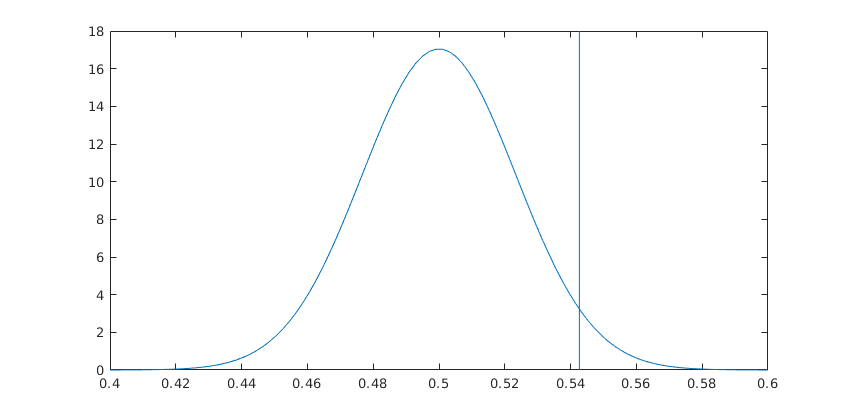
\includegraphics[scale=0.28]{fig1}
    \caption{Plot of null distribution}
\end{center}
\end{figure}
    \item The null hypothesis $H_0$ is that the probability of a competitor wearing red winning is equal to $0.5$. The alternative hypothesis $H_a$ is that the probability of the competitor wearing red winning is not equal to $0.5$.
        $$H_0: p = 0.5, \quad H_a: p \neq 0.5$$
    \item From \texttt{2*(1-normcdf(Z))} in Matlab, we get a p-value of $0.0681$ which is double the one-sided p-value.
    \item 
    \item Moving from a one-sided to a two-sided test increases the difficulty of rejecting the null hypothesis. This is because your p-value is doubled in a two-sided test. 

\end{enumerate}

\subsection{Effect size}%
\label{sub:Effect size}
\begin{enumerate}[label=\alph*.]
    \item 
\end{enumerate}

\subsection{Sample size}%
\label{sub:Sample size}
\begin{enumerate}[label=\alph*.]
    \item 
\end{enumerate}

\section{Sampling distribution}%
\label{sec:Sampling distribution}
\begin{enumerate}[label=\alph*.]
    \item 
\end{enumerate}


\section{Executive}%
\label{sec:Executive}
\begin{enumerate}[label=\alph*.]
    \item 
\end{enumerate}

\section{Lottery}%
\label{sec:Lottery}
\begin{enumerate}[label=\alph*.]
    \item 
\end{enumerate}

\section{Stomach flu}%
\label{sec:Stomach flu}
\begin{enumerate}[label=\alph*.]
    \item 
\end{enumerate}

\section{Matlab problem}%
\label{sec:Matlab problem}
\begin{enumerate}[label=\alph*.]
    \item 
\end{enumerate}

% \begin{figure}
% \begin{center}
%     \includegraphics[scale=0.28]{ps1_hist}
% \end{center}
% \end{figure}


\end{document}
